\begin{homeworkProblem}
  Descargue el archivo Datos.txt de la pagina del curso. En este encontrara un conjunto de 21 datos. Copie estos datos y calcule el polinomio de ajuste de grado 5 $p(x)=c_0+c_1x+c_2x^2+c_3x^3+c_4x^4+c_5x^5$ utilizando los métodos de ecuaciones normales y factorizacion $QR$. Compare sus resultados con los valores certificados $c_i=1$ para $i=0,1,\cdots,5$. Encuentre el residual $\|Ac-y\|_2$ en cada caso, así como la diferencia relativa con respecto a los valores certificados. Escriba sus conclusiones.
  \begin{solucion}
    \begin{enumerate}
      \item Usando Cholesky.\\
        \begin{lstlisting}[language = matlab]
format rational
n = 5; %Grado del polinómio
x = (0:1:20)';
y = [75901, -204794, 204863, -204436, 253665, -200894, 214131, -185192, 221249, -138370, 315911, -27644, 455253, 197434, 783995, 608816, 1370781, 1303798, 2205519, 2408860, 3444321]';

% Tomar tiempo de ejecución
tic;

% Construcción de la matriz Vandermonde
A = vander(x);
A = A(:, end-n:end); % Tomar las n+1 columnas necesarias

% Construcción de ecuaciones normales
B = A' * A;
z = A' * y;

% Descomposición de Cholesky
L = chol(B, 'lower'); % Matriz triangular inferior

% Resolver el sistema de ecuaciones
sol1chol = L \ z;      
solchol = L' \ sol1chol;
tiempo_chol = toc

% Mostrar solución final
disp(solchol);

xx = linspace(min(x), max(x), 100); % Puntos más finos para la curva
AA = xx(:).^(0:n); % Matriz de diseño para interpolación
yy = AA * solchol; % Evaluación del polinomio

plot(x, y, 'ro', 'MarkerSize', 8, 'DisplayName', 'Datos originales'); % Puntos originales
hold on;
plot(xx, yy, 'b-', 'LineWidth', 2, 'DisplayName', 'Polinomio ajustado'); % Polinomio
legend;
grid on;
title('Ajuste polinomial usando mínimos cuadrados con Cholesky');
xlabel('x');
ylabel('y');
hold off;
        \end{lstlisting}
        En dónde en un tiempo de $\frac{29}{77957}\approx 0.000372$ nos lista los coeficientes $c_i=1$ con $i=0,1,\cdots,5$ y la gráfica
        \begin{figure}[H]
          \begin{center}
            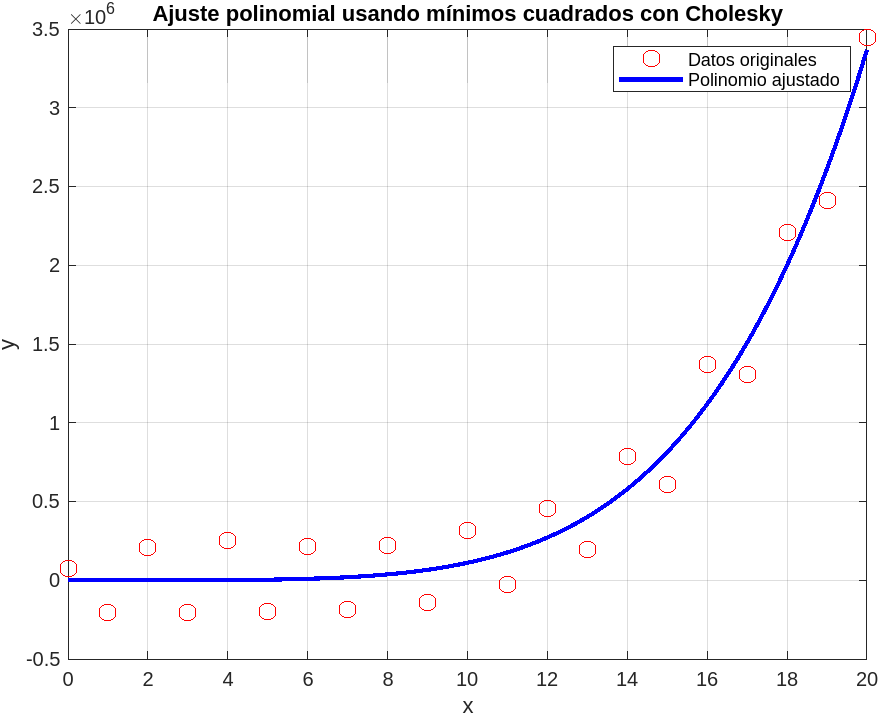
\includegraphics[scale=0.7]{Figures/choleskypunto2.png}
          \end{center}
          \caption{Usando el método de Cholesky.}
        \end{figure}
        \newpage
      \item Usando la factorización QR.\\
        \begin{lstlisting}[language = matlab]
format rational
n = 5; %Grado del polinómio
x = (0:1:20)';
y = [75901, -204794, 204863, -204436, 253665, -200894, 214131, -185192, 221249, -138370, 315911, -27644, 455253, 197434, 783995, 608816, 1370781, 1303798, 2205519, 2408860, 3444321]';

% Tomar tiempo de ejecución
tic;

% Construcción de la matriz Vandermonde
A = vander(x);
A = A(:, end-n:end); % Tomar las n+1 columnas necesarias

% Factorización QR
[Q,R] = qr(A);

% Ecuaciones QR

b = Q'*y;
solqr = R \ b;
tiempo_qr = toc

% Mostrar solución final
disp(solchol);

xx = linspace(min(x), max(x), 100); % Puntos más finos para la curva
AA = xx(:).^(0:n); % Matriz de diseño para interpolación
yy = AA * solchol; % Evaluación del polinomio

plot(x, y, 'ro', 'MarkerSize', 8, 'DisplayName', 'Datos originales'); % Puntos originales
hold on;
plot(xx, yy, 'b-', 'LineWidth', 2, 'DisplayName', 'Polinomio ajustado'); % Polinomio
legend;
grid on;
title('Ajuste polinomial usando factorización QR');
xlabel('x');
ylabel('y');
hold off;
        \end{lstlisting}
        En dónde en un tiempo de $\frac{47}{125000}s\approx 0.000376 s$ nos lista los coeficientes $c_i=1$ con $i=0,1,\cdots,5$ y la gráfica 
        \begin{figure}[H]
          \begin{center}
            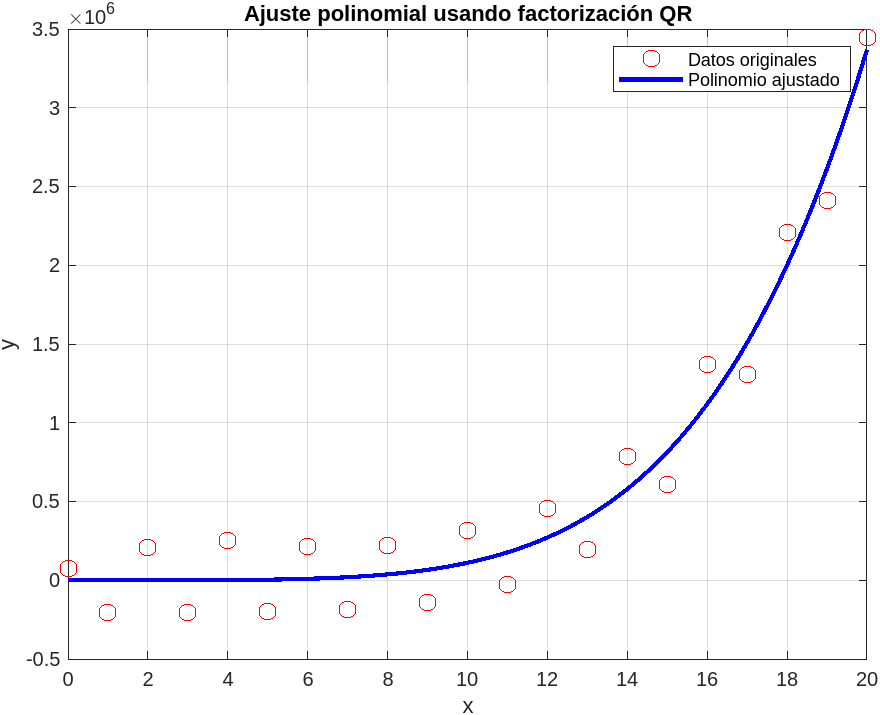
\includegraphics[scale=0.7]{Figures/qrpunto2.png}
          \end{center}
          \caption{Usando el método de factorización QR.}
        \end{figure} 
    \end{enumerate}
    \textbf{Conclusiones:} experimentalmente ambos métodos parecen dar de manera explícita los valores certificados, por lo que sería más objetivo hablar sobre el tiempo de ejecución del método en matlab, lo que vimos anteriormente que le da el punto al método de Cholesky, pues este tuvo un tiempo de ejecución menor al de la factorización QR. Por otro lado, la diferencia relativa con respecto a los valores certificados en ambos casos es de $0$ al ser idénticos a los valores dados en el problema, veamos por otro lado el residual:
    \begin{align*}
      \|Ac_{chol}-y\|_{2}&=914080\\
      \|Ac_{QR}-y\|_{2}&= 914080
    \end{align*}
    Esto se explica al ambos métodos llegar a la misma solución.\\
    En fin, si bien en este experimento parece que el método de Cholesky es más eficiente que el método de factorización $QR$, recordemos que teóricamente el método $QR$ tiene mayor estabilidad que Cholesky por el número de condición que se plantea en ambos casos, por lo que es válido pensar que para polinomios de grado mucho mayor lo sucedido en este experimento no siga sucediendo. 
  \end{solucion}
\end{homeworkProblem}
